\documentclass[12pt, twoside]{article}
\usepackage[letterpaper, margin=1in, headsep=0.5in]{geometry}
\usepackage[english]{babel}
\usepackage[utf8]{inputenc}
\usepackage{amsmath}
\usepackage{amsfonts}
\usepackage{amssymb}
\usepackage{tikz}
\usetikzlibrary{quotes, angles}
\usepackage{graphicx}
\usepackage{multicol}

%\usepackage{pgfplots}
%\pgfplotsset{width=10cm,compat=1.9}
%\usepgfplotslibrary{statistics}
%\usepackage{pgfplotstable}
%\usepackage{tkz-fct}
%\usepackage{venndiagram}

\usepackage{fancyhdr}
\pagestyle{fancy}
\fancyhf{}
\renewcommand{\headrulewidth}{0pt} % disable the underline of the header

\fancyhead[RE]{\thepage}
\fancyhead[RO]{\thepage \\ Name: \hspace{3cm}}
\fancyhead[L]{BECA / Dr. Huson / Geometry 10th Grade\\* Unit 2: Midpoints and distance \\ 
26 September 2019}

\begin{document}
  \subsubsection*{2.8 Do Now: Constructions}

  \begin{enumerate}
    \item Complete the construction of an equilateral triangle with one side as $\overline{AB}$. \vspace{3cm}
    \begin{center}
    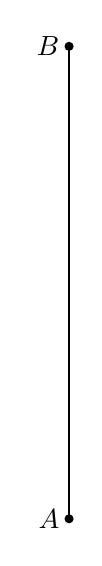
\begin{tikzpicture}
      \draw [-, thick] (0,0)--(0,6);
      \draw [fill] (0,0) circle [radius=0.05] node[left]{$A$};
      \draw [fill] (0,6) circle [radius=0.05] node[left]{$B$};
    \end{tikzpicture}
    \end{center} \vspace{3cm}
    \begin{enumerate}
      \item Identify two circles in the construction. For each, name the center of the circle and the radius.  \vspace{3cm}
      \item Assuming that the third vertex of the triangle is point $C$, explain why the distance from $A$ to $C$ is the same as the distance from $A$ to $B$.
    \end{enumerate}

  \newpage

    \item Complete the construction of a perpendicular bisector of $\overline{AB}$. Label the midpoint $M$. \vspace{2cm}
    \begin{center}
    \begin{tikzpicture}
      \draw [-, thick] (0,0)--(-2,6);
      \draw [fill] (0,0) circle [radius=0.05] node[below right]{$A$};
      \draw [fill] (-2,6) circle [radius=0.05] node[above left]{$B$};
    \end{tikzpicture}
    \end{center} \vspace{3cm}

    \subsubsection*{Early finishers: Solve for $x$ by factoring}
    \begin{multicols}{2}
    \item $x^2+6x+5=0$
    \item $x^2+5x=14$
    \end{multicols}


\end{enumerate}
\end{document}
